\documentclass[12pt, a4paper]{report}

\usepackage[utf8]{inputenc}
\usepackage[T1]{fontenc}
\usepackage[english]{babel}
\usepackage{geometry}
\geometry{a4paper, margin=1in, headheight=14.5pt} % Adjusted margins with proper headheight
\usepackage{pdfpages}
\usepackage{emptypage} % To ensure blank pages are truly empty
\usepackage{microtype} % Improve justification and reduce overfull hboxes
\usepackage{titlesec} % For custom chapter and section styling
\usepackage{xcolor} % For custom colors
\usepackage[most]{tcolorbox} % For colored boxes
\usepackage{fancyhdr} % For custom headers and footers
\usepackage{tocloft} % For Table of Contents customization
\usepackage{lettrine} % For drop caps
\usepackage{lipsum} % For dummy text if needed
\usepackage{enumitem} % For better list control
\usepackage{caption} % For caption styling
\usepackage{setspace} % For line spacing control
\usepackage{pifont} % For decorative symbols
\usepackage{tikz} % For drawing fancy elements
\usepackage{amssymb} % For mathematical symbols like \checkmark
\usepackage{bookmark} % Better PDF bookmarks
\usepackage{hyperref} % For clickable links in ToC (moved to after other packages)
\usepackage{float}
\usepackage{colortbl} % For colored table cells
\usepackage{array} % For better table column formatting
\usepackage{calc} % For coordinate calculations in TikZ
\usepackage{mdframed} % For framed environments
\usepackage{afterpage} % For operations on the following page
\usetikzlibrary{calc}
\tcbuselibrary{skins,breakable}

% Define a refined professional color palette
\definecolor{primary}{RGB}{33, 64, 95} % Deep navy blue
\definecolor{secondary}{RGB}{145, 145, 145} % Medium gray
\definecolor{accent}{RGB}{201, 172, 140} % Gold/Bronze accent
\definecolor{background}{RGB}{248, 248, 248} % Light background
\definecolor{bodytext}{RGB}{40, 40, 40} % Near-black for body text

% Set default text color
\color{bodytext}

% Customize chapter style - more elegant
\titleformat{\chapter}[display]
{\normalfont\Large\bfseries\color{primary}}
{\filcenter\color{primary}\MakeUppercase{\chaptertitlename}~\thechapter}
{1em}
{\filcenter\LARGE}[\vspace{0.5em}\centerline{\rule{0.6\textwidth}{1pt}}]
\titlespacing*{\chapter}{0pt}{30pt}{40pt}

% Section styling - more subtle
\titleformat{\section}
{\normalfont\large\bfseries\color{primary}}
{\thesection}{1em}{}
\titlespacing*{\section}{0pt}{3.5ex plus 1ex minus .2ex}{2.3ex plus .2ex}

% Subsection styling
\titleformat{\subsection}
{\normalfont\normalsize\bfseries\color{primary}}
{\thesubsection}{1em}{}

% Set up fancy headers - more elegant
\pagestyle{fancy}
\fancyhf{}
\fancyhead[R]{\thepage}
\fancyhead[L]{\textit{\leftmark}}
\fancyfoot[C]{\textcolor{secondary}{\small{Final Year Project}}}
\renewcommand{\headrulewidth}{0.4pt}
\renewcommand{\footrulewidth}{0.2pt}

% Enhanced Table of Contents styling
% Title formatting
\renewcommand{\cfttoctitlefont}{\hfill\LARGE\bfseries\color{primary}} 
\renewcommand{\cftaftertoctitle}{\hfill\null\\[1em]\hfill\rule{0.6\textwidth}{1pt}}

% Entry formatting
\renewcommand{\cftchapfont}{\normalfont\bfseries\color{bodytext}} % Chapter font in black
\renewcommand{\cftsecfont}{\normalfont\itshape} % Section font
\renewcommand{\cftsubsecfont}{\normalfont} % Subsection font

% Dot leaders with custom styling
\renewcommand{\cftdot}{$\cdot$} % Better centered dots
\renewcommand{\cftdotsep}{2.0} % Tighter dot spacing
\renewcommand{\cftchapleader}{\color{secondary}\cftdotfill{\cftdotsep}} % Chapter dots
\renewcommand{\cftsecleader}{\color{secondary}\cftdotfill{\cftdotsep}} % Section dots

% Page numbers
\renewcommand{\cftchappagefont}{\normalfont\bfseries\color{bodytext}} % Chapter page number
\renewcommand{\cftsecpagefont}{\normalfont\color{bodytext}} % Section page number

% Spacing for better presentation
\setlength{\cftbeforetoctitleskip}{1em} % Space before title
\setlength{\cftaftertoctitleskip}{2em} % Space after title
\setlength{\cftbeforechapskip}{1em} % Space before chapters
\setlength{\cftbeforesecskip}{0.5em} % Space before sections

% Chapter numbering format
\renewcommand{\cftchappresnum}{\color{primary}} % Color for chapter numbers
\renewcommand{\cftchapaftersnum}{.\hspace{0.8em}} % Add period after number

% Indentation
\setlength{\cftchapindent}{0em} % No indent for chapters
\setlength{\cftsecindent}{1.5em} % Indent for sections
\setlength{\cftsubsecindent}{3em} % Indent for subsections

% Title
\renewcommand{\contentsname}{\color{primary}Table of Contents}

% Improved caption style
\captionsetup{
  font=small,
  labelfont={bf,color=primary},
  margin=10pt,
  format=hang,
  justification=centering,
}

% Lettrine (drop caps) settings - more elegant
\renewcommand{\LettrineFontHook}{\color{primary}\bfseries}
\setcounter{DefaultLines}{3}
\setlength{\DefaultFindent}{0.5em}
\setlength{\DefaultNindent}{0em}
\setlength{\DefaultSlope}{0pt} % Ensure proper alignment

% Define line spacing for main text
\onehalfspacing

% Hyperref settings - more professional
\hypersetup{
    colorlinks=true,
    linkcolor=primary,
    filecolor=primary,
    urlcolor=primary,
    citecolor=primary,
    pdftitle={PFE Rapport},
    pdfauthor={KORPOR},
    pdfsubject={Final Year Project},
    pdfkeywords={MySQL, Express-Node.js, React, Vite},
    pdfpagemode=UseOutlines,
    pdfstartview=FitH,
    bookmarksopen=true,
    bookmarksnumbered=true,
}

% Define a new environment for important information - more elegant
\newenvironment{important}{%
  \begin{tcolorbox}[
    colback=background,
    colframe=primary,
    arc=1mm, % Slightly rounded corners
    boxrule=0.5pt,
    left=8pt,
    right=8pt,
    top=6pt,
    bottom=6pt,
    width=\textwidth,
    title={\textbf{Important}},
    fonttitle=\color{white}
  ]
}{%
  \end{tcolorbox}
}

% Define a command for first paragraph styling with better alignment
\newcommand{\firstparagraph}[1]{%
  \lettrine[lines=2,findent=0.5em,nindent=0em,loversize=0.05,lraise=0.05]{\textcolor{primary}{#1}}{}%
}

% Define a command for chapter quotes
\newcommand{\chapterquote}[2]{%
  \begin{flushright}
    \begin{minipage}{0.7\textwidth}
      \small\itshape #1
      \begin{flushright}
        \normalfont --- #2
      \end{flushright}
    \end{minipage}
  \end{flushright}
  \vspace{1cm}
}

% Enhanced figure environment with side lines
\newtcolorbox{figureframe}{
  enhanced,
  frame hidden,
  boxrule=0mm,
  borderline west={3.5pt}{0pt}{primary},
  sharp corners,
  breakable,
  left=15pt,
  right=0pt,
  top=0pt,
  bottom=0pt,
  toptitle=0pt,
  bottomtitle=0pt,
  colback=white,
  overlay={
    % Main accent line
    \draw[line width=1pt, accent] ([xshift=5pt]frame.north west) -- ([xshift=5pt]frame.south west);
    
    % Top decorative elements
    \fill[accent] ([xshift=0pt,yshift=-3pt]frame.north west) circle (2pt);
    \draw[line width=0.75pt, accent] ([xshift=7pt,yshift=-5pt]frame.north west) -- ([xshift=15pt,yshift=-5pt]frame.north west);
    
    % Bottom decorative elements
    \fill[accent] ([xshift=0pt,yshift=3pt]frame.south west) circle (2pt);
    \draw[line width=0.75pt, accent] ([xshift=7pt,yshift=5pt]frame.south west) -- ([xshift=15pt,yshift=5pt]frame.south west);
  }
}

\let\origfigure\figure
\let\endorigfigure\endfigure

\renewenvironment{figure}[1][htbp]{%
  \origfigure[#1]%
  \begin{figureframe}%
}{%
  \end{figureframe}%
  \endorigfigure%
}

% Styled table environment with decorative side line - same style
\newtcolorbox{tableframe}{
  enhanced,
  frame hidden,
  boxrule=0mm,
  borderline west={3.5pt}{0pt}{primary},
  sharp corners,
  breakable,
  left=15pt,
  right=0pt,
  top=0pt,
  bottom=0pt,
  toptitle=0pt,
  bottomtitle=0pt,
  colback=white,
  overlay={
    % Main accent line
    \draw[line width=1pt, accent] ([xshift=5pt]frame.north west) -- ([xshift=5pt]frame.south west);
    
    % Top decorative elements
    \fill[accent] ([xshift=0pt,yshift=-3pt]frame.north west) circle (2pt);
    \draw[line width=0.75pt, accent] ([xshift=7pt,yshift=-5pt]frame.north west) -- ([xshift=15pt,yshift=-5pt]frame.north west);
    
    % Bottom decorative elements
    \fill[accent] ([xshift=0pt,yshift=3pt]frame.south west) circle (2pt);
    \draw[line width=0.75pt, accent] ([xshift=7pt,yshift=5pt]frame.south west) -- ([xshift=15pt,yshift=5pt]frame.south west);
  }
}

\let\origtable\table
\let\endorigtable\endtable
\renewenvironment{table}[1][htbp]{%
  \origtable[#1]%
  \begin{tableframe}%
}{%
  \end{tableframe}%
  \endorigtable%
}

\begin{document}

% Cover Page

\includepdf[pages=1]{cover page.pdf}

% Blank Page after Cover - ensure it's actually blank
\newpage
\thispagestyle{empty}
\null
\newpage

% Start Arabic page numbering
\pagenumbering{arabic}

% Summary and Abstract
% Summary and Abstract on the same page
\thispagestyle{empty} % Remove page style for this page

% Create a more elegant title for Summary
\begin{center}
{\color{primary}\Large\textbf{\MakeUppercase{Summary}}}
\end{center}
\vspace{0.1cm}
\begin{center}
\rule{0.6\textwidth}{1pt}
\end{center}
\vspace{0.5cm}
\addcontentsline{toc}{chapter}{Summary}

\noindent \firstparagraph{T}his work is part of the completion of our Final Year Project at the Higher Institute of Computer Science and Mathematics of Monastir for the academic year 2024-2025, aiming for the National Fundamental License Diploma in Computer Science. Conducted within the company \textbf{\textcolor{primary}{'KZ IT Services'}}, our main objective is the development of a mobile application and a web back-office dedicated to real estate investment named \textbf{\textcolor{primary}{'KORPOR'}}. We used MySQL to manage the databases, Express-Node.js to implement the backend, and React and Vite to implement the frontend. Project management followed the SCRUM Agile methodology, emphasizing agile practices such as sprint planning, sprint management, and regular meetings.

% Keywords in a more professional design
\vspace{0.3cm}
\begin{tcolorbox}[
    colback=background,
    colframe=primary,
    arc=1mm,
    boxrule=0.5pt,
    left=8pt,
    right=8pt,
    top=4pt,
    bottom=4pt,
    width=\textwidth
]
\textbf{Keywords:} MySQL, Express-Node.js, React, Vite.
\end{tcolorbox}

\vspace{1.2cm} % Space between sections

% Horizontal rule to separate sections
\begin{center}
\textcolor{secondary}{\rule{0.7\textwidth}{0.5pt}}
\end{center}

\vspace{1.2cm}

% Create a more elegant title for Abstract
\begin{center}
{\color{primary}\Large\textbf{\MakeUppercase{Abstract}}}
\end{center}
\vspace{0.1cm}
\begin{center}
\rule{0.6\textwidth}{1pt}
\end{center}
\vspace{0.5cm}
\addcontentsline{toc}{chapter}{Abstract}

\noindent \firstparagraph{T}his project is part of our graduation project at the Higher Institute of Computer Science and Mathematics of Monastir for the 2024-2025 academic year, leading to the national diploma of fundamental license in Computer Science.
Carried out within the company \textbf{\textcolor{primary}{"KZ IT Services"}}, our main objective is the development of a mobile application and web back office dedicated to real estate investment called \textbf{\textcolor{primary}{"KORPOR"}}. We used MySQL to manage the databases, Express-Node.js for the backend implementation, and React and Vite for the frontend.
The project management followed the SCRUM Agile methodology, with an emphasis on agile practices such as sprint planning, sprint management, and regular meetings.

% Keywords in a more professional design
\vspace{0.3cm}
\begin{tcolorbox}[
    colback=background,
    colframe=primary,
    arc=1mm,
    boxrule=0.5pt,
    left=8pt,
    right=8pt,
    top=4pt,
    bottom=4pt,
    width=\textwidth
]
\textbf{Keywords:} MySQL, Express-Node.js, React, Vite.
\end{tcolorbox}

% Ensure Summary and Abstract stay on the same page
\nopagebreak 
\cleardoublepage

% Dedication
\chapter*{\centering Dedication}
\addcontentsline{toc}{chapter}{Dedication}

\begin{center}
{\itshape\large 
To the memory of my beloved father, whose guidance and wisdom continue to light my path. \\
Though no longer with us, your presence remains in every achievement of my life.

\vspace{0.8cm}

To my loving mother, whose strength and endless support shaped who I am today.

\vspace{0.8cm}

To my sister and brother, whose companionship and encouragement \\
have been constant sources of joy and motivation.

\vspace{0.8cm}

To my little Aryouma, whose innocence and love bring happiness to our family every day.

\vspace{0.8cm}

To Mme Nadia, my professors and mentors, who have guided me \\
with knowledge and patience throughout my academic journey.

\vspace{0.8cm}

To my friends, whose encouragement made this journey worthwhile.

\vspace{0.8cm}

\textbf{This work is dedicated to all of you, but especially to you, Father.}
}
\end{center}

\vspace{0.5cm}

% \begin{center}
% 
\includegraphics[width=0.2\textwidth]{images/qr-code-dedication.png}
% \end{center}

% \vspace{1cm}

\begin{flushright}
    \begin{minipage}{0.4\textwidth}
        \centering
        
\includegraphics[width=1\textwidth]{images/Ahmed jaziri signature.png}\\
    \end{minipage}
\end{flushright}

\thispagestyle{empty} 
\cleardoublepage

% Acknowledgement
\chapter*{\centering Acknowledgement}
\addcontentsline{toc}{chapter}{Acknowledgement}
% Add your Acknowledgement content here later 
\cleardoublepage

% Table of Contents with enhanced styling
\thispagestyle{empty}

% Decorative frame for TOC page
\begin{tikzpicture}[remember picture, overlay]
  % Draw a subtle decorative line at top of page
  \draw[color=accent, line width=0.5pt] 
    ([yshift=-1.5cm]current page.north west) -- 
    ([yshift=-1.5cm]current page.north east);
  % Draw a matching line at bottom of page  
  \draw[color=accent, line width=0.5pt] 
    ([yshift=1.5cm]current page.south west) -- 
    ([yshift=1.5cm]current page.south east);
\end{tikzpicture}

\begin{center}
{\color{primary}\LARGE\textbf{\MakeUppercase{Table of Contents}}}

% Decorative element below title
\begin{tikzpicture}
  \draw[color=primary, line width=1pt] (0,0) -- (6,0);
  \draw[color=accent, line width=0.5pt] (1,0.15) -- (5,-0.15);
\end{tikzpicture}
\end{center}
% \vspace{1.8cm}

% Hide the default "Contents" heading and remove any default horizontal line
\renewcommand{\contentsname}{}
\renewcommand{\cftaftertoctitle}{}

\begin{minipage}{\textwidth}
\begingroup
\fontsize{11pt}{13pt}\selectfont
\tableofcontents
\endgroup
\end{minipage}

% Ensure TOC pages have no page numbers
\addtocontents{toc}{\protect\thispagestyle{empty}}

% Add this to make sure the second TOC page also has no page number
\addtocontents{toc}{\protect\afterpage{\protect\thispagestyle{empty}}}

\cleardoublepage

% General Introduction
\thispagestyle{empty}

\vspace*{\fill}

\begin{center}
\begin{minipage}{1\textwidth}
    \begin{center}
        \large\itshape ``Real estate cannot be lost or stolen, nor can it be carried away. Purchased with common sense, paid for in full, and managed with reasonable care, it is about the safest investment in the world.''\cite{RooseveltRealEstateQuote}
        \vspace{1cm}
        
        \normalfont\textcolor{primary}{— Franklin D. Roosevelt}\\
        \small\textcolor{secondary}{32nd President of the United States}
    \end{center}
\end{minipage}
\end{center}

\vspace*{\fill}

\newpage
\thispagestyle{empty}

\chapter*{\centering General Introduction}
\addcontentsline{toc}{chapter}{General Introduction}
\vspace{-1cm} % Reduce space after title

% \vspace{0.1cm}
% \begin{center}
% % \rule{0.6\textwidth}{1pt}
% \end{center}
% \vspace{0.3cm}

% \vspace{1cm}

\begingroup % Begin group to localize changes
\setlength{\parindent}{0pt} % Remove paragraph indentation
\setlength{\parskip}{0.15em} % Reduce space between paragraphs even more
\footnotesize % Smaller font size to fit on one page

\firstparagraph{I}n today's rapidly evolving financial landscape, traditional investment methods are often burdened by opaque processes, cumbersome bureaucracy, and significant entry barriers. Investors have long struggled with outdated systems that impede transparency, elevate risks, and complicate access to promising opportunities. Such challenges not only limit diversification but also expose users to uncertainties that modern technology can easily overcome.

\noindent \textbf{\textcolor{primary}{Korpor}} was conceived to transform this paradigm by delivering a fully integrated, AI and blockchain-powered mobile investment platform. By harnessing advanced data analytics, machine learning, and cutting-edge blockchain technology, Korpor streamlines every facet of the investment process. The application offers a seamless user onboarding experience, intuitive project listings enriched with AI-driven recommendations, and a secure, automated investment flow that simplifies transactions while ensuring that every operation is recorded immutably on the blockchain. Investors can manage their portfolios effortlessly through a comprehensive dashboard, with real-time notifications, an interactive AI chatbot, and multi-language support delivering a personalized and globally accessible experience.

\noindent \textbf{\textcolor{primary}{Security and trust}} are at the heart of Korpor's design. By employing state-of-the-art encryption, blockchain-based transparency, and strict compliance measures, the platform safeguards sensitive financial data and guarantees that every transaction is executed within a secure and verifiable framework. Continuous monitoring, performance optimization, and the immutable nature of blockchain records further ensure that the application remains resilient, scalable, and resistant to fraud in a dynamic market environment.

\noindent Developed under a flexible Agile framework that combines iterative development with strategic project management best practices, Korpor is designed to rapidly adapt to evolving market trends and user needs. This methodical approach allows for regular feedback, swift enhancements, and the seamless integration of innovative features throughout the development lifecycle.


% Our document is structured as follows:

% \vspace{-0.4cm} % Reduce space before list
\begin{itemize}[leftmargin=1.5em, itemsep=0pt, parsep=0pt, topsep=0.05cm]
\item The first chapter, \textbf{\textcolor{primary}{Project Context}}, delves into the industry challenges and the vision that inspired Korpor's creation.
\item The second chapter, \textbf{\textcolor{primary}{Analysis and Specification of Needs}}, outlines the comprehensive requirements gathering, needs analysis, architectural design, and the selection of cutting-edge tools and technologies.
\item Subsequent chapters document the progressive implementation of core features—from AI-enhanced project recommendations and blockchain-secured transactions to comprehensive portfolio management—each developed through clearly defined sprints encompassing analysis, design, and deployment phases.
\end{itemize}

\vspace{0.05cm}
\noindent Through this structured approach, we demonstrate how Korpor leverages modern technology to reimagine investment management, offering a secure, transparent, and dynamic solution that is set to redefine digital financial engagement.

\endgroup % End group to restore normal settings
\enlargethispage{4cm} % Allow this page to be longer
\cleardoublepage

% Chapter 1: Project Context
\chapter{Project Context}

\section{Introduction}

The aim of this chapter is to present the general framework of the Korpor project, a solution dedicated to real estate investment. In this section, we'll discuss successively:

\begin{itemize}
    \item The presentation of the host organization.
    \item The context and challenges of the real estate sector.
    \item Analysis of existing solutions and identification of their limitations.
    \item Definition of functional and non-functional needs of the mobile application and web back office.
\end{itemize}

\section{Project Context}

This work is part of the end-of-study project for the national diploma of Applied Bachelor's degree in Computer Science from the Higher Institute of Computer Science and Mathematics of Monastir (ISIMM) for the year 2024/2025. I had the opportunity to do my end-of-study internship at the company
``KZ IT Services'', under the supervision of Mr. Khalil Zouari.

\section{Hosting Company}

The purpose of this section is to present the company within which I developed my project, as shown in Figure \ref{fig:hosting-company}.

\begin{figure}[htbp]
    \centering
    
\includegraphics[width=0.2\textwidth]{images/company-logo.png}
    \caption{Hosting Company ``KZ IT Services''}
    \label{fig:hosting-company}
\end{figure}

\subsection{Hosting Company}

\textbf{\textcolor{primary}{KZ IT Service}} is a dynamic software company dedicated to delivering innovative IT solutions tailored to modern business needs. We specialize in designing and developing robust, scalable applications that drive efficiency and digital transformation. Our experienced team leverages cutting-edge technology to create customized software that exceeds client expectations. With a strong commitment to quality and continuous improvement, we build lasting partnerships based on trust and excellence. At ``KZ IT Service'', innovation is at the core of everything we do, empowering our clients to achieve sustainable growth and success.

\section{Preliminary Study}

This preliminary study provides a review of some existing investment and asset management platforms. Further, the next section identifies some key concepts that will lead to further understanding of the domain in question.

\subsection{Existing Solutions Study}

For understanding the present scenario and to clearly demarcate our goals, some renowned investment platform analyses offering similar features, including ``Aseel'' and ``Stake'', are performed \cite{G2CompetitiveAnalysis2024, AsanaCompetitiveAnalysis2024}.

\subsection{Available solutions and analysis}

\subsubsection{The Aseel Platform}

\textbf{\textcolor{primary}{Aseel}} is a portal through which users can invest in different real estate projects with ease. The interface allows the clients to surf various investment opportunities, view the details of the properties, and then make an informed decision. Aseel introduces transparency in the investment process by offering financial data, updates regarding projects, and returns that are estimated. This platform comes with an easy-to-use dashboard through which one tracks their investments and manages their assets without any hassle. The interface of the Aseel Platform is shown in Figure \ref{fig:aseel-platform}.

\newpage

\begin{figure}[htbp]
    \centering
    
\includegraphics[width=0.65\textwidth]{images/Interface-of-the Aseel Platform.png}
    \caption{Interface of ``The Aseel Platform''}
    \label{fig:aseel-platform}
\end{figure}

\begin{center}
    \vspace{0.5em}
    \begin{tikzpicture}
        \draw[primary, line width=1pt] (0,0) -- (0.3\textwidth,0);
        \draw[accent, line width=0.7pt] (0.1\textwidth,-0.07) -- (0.4\textwidth,0.07);
        \fill[primary] (0,0) circle (2pt);
        \fill[accent] (0.3\textwidth,0) circle (2pt);
    \end{tikzpicture}
    \vspace{0.5em}
\end{center}

\subsubsection{The Stake Platform}

\textbf{\textcolor{primary}{Stake}} is an online investment platform that deals with real estate crowdfunding. It provides the opportunity to invest in fractions of property ownership, hence diversifying a portfolio without huge capital. On Stake, there are AI-powered recommendations based on user preferences, seamless payment integration, and a secure environment for investment. Besides, liquidity is guaranteed by enabling exit options for investors who may want to sell their shares in ongoing projects. Figure \ref{fig:stake-platform} illustrates the interface of the Stake Platform.

\newpage
\thispagestyle{empty}
\newpage

\begin{figure}[htbp]
    \centering
    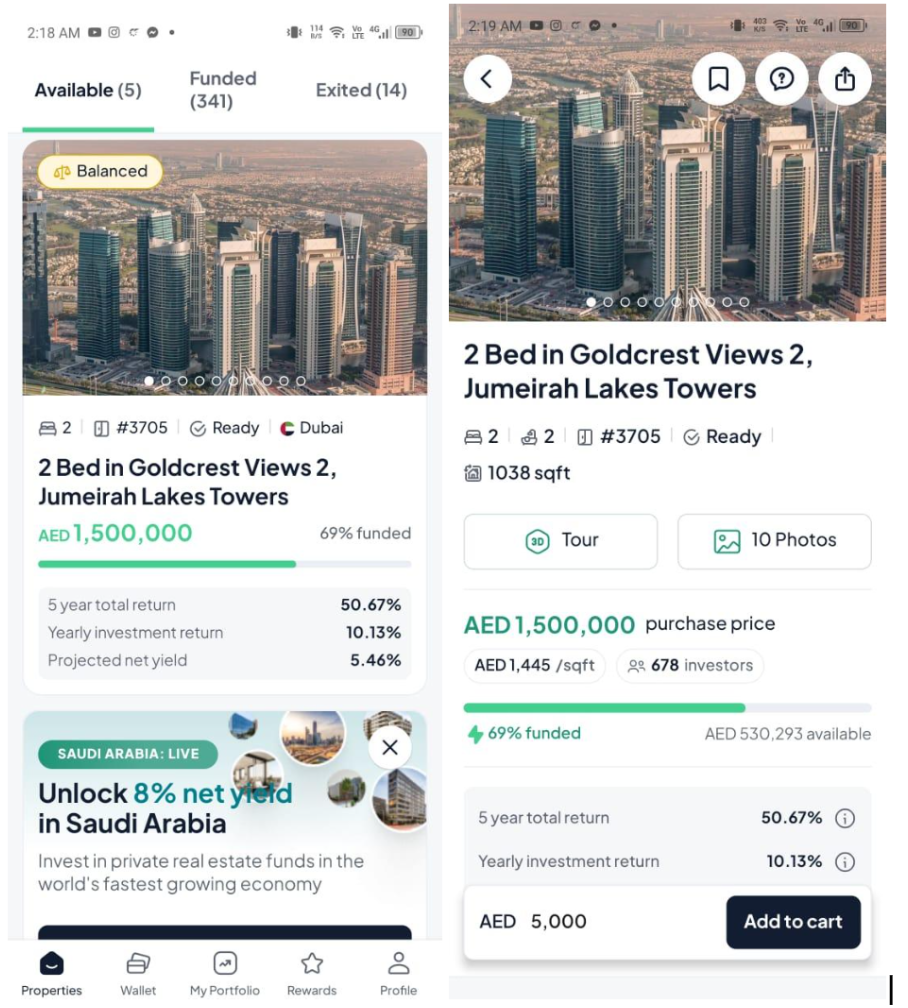
\includegraphics[width=0.65\textwidth]{images/Interface-of-the Stake Platform.png}
    \caption{Interface of ``The Stake Platform''}
    \label{fig:stake-platform}
\end{figure}

\subsection{Comparative and Critical Analysis}

We can summarize all that comes from our analysis based on a number of criteria used for the evaluation of these applications \cite{LyssnaUXAnalysis2024, StrategicManagementInsightCA2024}.

\begin{itemize}
    \item \textbf{Speed (C1)}: The platform should obtain value for the user as fast as possible and effectively, anticipating their proliferating expectations.
    \item \textbf{Costs (C2)}: With minimum software development costs, it is important to keep the pricing predictable and acceptable.
    \item \textbf{Quality (C3)}: Since the market expects quality, any kind of error might affect brand reputation. Improvement of the platform should be regular.
    \item \textbf{Reliability (C4)}: Since modern-day investment platforms need to make sure of minimum downtime and maximum availability of services, this factor is critical.
    \item \textbf{Security (C5)}: Such an investment platform enforces access rights, roles, and contribution rights through a powerful security system.
    \item \textbf{Performance (C6)}: Crucial features include AI-powered recommendations going through seamlessly, easy transaction tracking, and investment monitoring.
    \item \textbf{Stability (C7)}: The platform should have a proven track record, regular updates, and a large user base to ensure its longevity.
    \item \textbf{Resilience (C8)}: In order to prevent data loss and guarantee a smooth experience for investors, it must be able to restore lost functionalities should issues occur.
    \item \textbf{User Experience (C9)}: The interface should be intuitive and user-friendly, hence allowing investors to move with ease through it, thus making wiser decisions.
\end{itemize}

Table \ref{tab:evaluation} presents the evaluation of the existing solutions based on these criteria:

\begin{table}[htbp]
    \centering
    \caption{Evaluation Table}
    \label{tab:evaluation}
    \renewcommand{\arraystretch}{1.3}
    \begin{tabular}{|>{\columncolor{background}}c|*{9}{>{\centering\arraybackslash}p{0.7cm}|}}
        \hline
        \rowcolor{primary!15}
        \textcolor{primary}{\textbf{Solution}} & 
        \textcolor{primary}{\textbf{C1}} & 
        \textcolor{primary}{\textbf{C2}} & 
        \textcolor{primary}{\textbf{C3}} & 
        \textcolor{primary}{\textbf{C4}} & 
        \textcolor{primary}{\textbf{C5}} & 
        \textcolor{primary}{\textbf{C6}} & 
        \textcolor{primary}{\textbf{C7}} & 
        \textcolor{primary}{\textbf{C8}} & 
        \textcolor{primary}{\textbf{C9}} \\
        \hline
        \textbf{Stake} & \textcolor{primary}{\checkmark} & \textcolor{primary}{\checkmark} & \textcolor{primary}{\checkmark} & \textcolor{primary}{\checkmark} & \textcolor{primary}{\checkmark} & $\times$ & \textcolor{primary}{\checkmark} & \textcolor{primary}{\checkmark} & \textcolor{primary}{\checkmark} \\
        \hline
        \rowcolor{background!50}
        \textbf{Aseel} & \textcolor{primary}{\checkmark} & \textcolor{primary}{\checkmark} & \textcolor{primary}{\checkmark} & $\times$ & \textcolor{primary}{\checkmark} & $\times$ & \textcolor{primary}{\checkmark} & $\times$ & \textcolor{primary}{\checkmark} \\
        \hline
    \end{tabular}
\end{table}

\subsection{Proposed Solution}

Having studied the already working platforms for investments, we found strengths and weaknesses that could define what was required from the project. Our proposed solution will look at:

\begin{itemize}
    \item Developing an efficient mobile application for investment management.
    \item Increasing the level of users' engagement with recommendations using the power of AI \cite{MobileRealityAIRealEstate2024, HouseCanaryAIInvestors2024, SmilkovTensorFlowJS2019}.
    \item Ensuring responsive and user-friendly interaction with the interface.
    \item Gaining the trust of investors by ensuring transparency and security in the investing platform.
    \item Enhancing the security of data and following all the financial regulations.
\end{itemize}

The \textbf{\textcolor{primary}{Korpor}} platform will be offering the following features:

\begin{itemize}
    \item A directory of investment opportunities with deep financial insights into those opportunities.
    \item AI-driven recommendations of investments as per users' preferences \cite{LinkedInAIFinTech2024}.
    \item Smooth funding and payout mechanisms.
    \item Real-time portfolio performance tracking on a single screen/dashboard.
    \item Forum for interactive discussions on strategy and market trends among its users.
    \item Referral and Rewards System: An engaging system for rewarding users via referral.
\end{itemize}

\section{Development methodology}

The completion of the project on its delivery date is the main problem of every software development team. One of the most common problems encountered in the production of software is insufficient technical specifications, poor time management in the face of the use of emerging technology, and sudden changes in needs. In order to avoid these critical issues, we follow an agile methodology for project management, using tools like Git \cite{GitWebsite} for version control and GitHub \cite{GithubWebsite} for collaborative development.

\subsection{SCRUM}

\textbf{\textcolor{primary}{Scrum}} is an agile development approach that is used to create software using incremental and iterative methods. Scrum is a quick, flexible, and efficient agile methodology that is intended to provide value to the client at every stage of the project's development \cite{ScrumGuide2020}. Scrum is founded on empiricism and lean thinking, employing an iterative, incremental approach guided by the three pillars of transparency, inspection, and adaptation \cite{AtlassianScrumPillars, ScrumGuide2020}. Scrum's main goal is to meet customer needs by fostering an atmosphere of open communication, group accountability, and constant improvement, underpinned by the Scrum values of Commitment, Focus, Openness, Respect, and Courage \cite{ScrumGuide2020}. The development process begins with a broad concept of what must be constructed, developing a list of features that the product owner desires, and arranging them according to priority (product backlog).

\subsection{Agile Scrum roles and responsibilities}

\subsubsection{The Product Owner}

Understands the customer and business requirements, then creates and manages the product backlog based on those requirements.

\textbf{Responsibilities:}
\begin{itemize}
    \item Managing the scrum backlog
    \item Release management
    \item Stakeholder management
\end{itemize}

\subsubsection{Developers}

In Scrum, the term developer or team member refers to anyone who plays a role in the development and support of the product and can include researchers, architects, designers, programmers, etc.

\textbf{Responsibilities:}
\begin{itemize}
    \item Delivering the work through the sprint
    \item To ensure transparency during the sprint, they meet daily at the daily scrum
\end{itemize}

\subsubsection{Scrum Master}

The role responsible for gluing everything together and ensuring that scrum is being done well. In practical terms, that means they help the product owner define value, the development team deliver the value, and the scrum team get better.

The Scrum Master focuses on:
\begin{itemize}
    \item Transparency
    \item Empiricism
    \item Self-organization
    \item The Scrum events
\end{itemize}

\subsection{The Scrum Events}

The Scrum events are key elements of the Scrum Framework. They provide regular opportunities for enacting the Scrum pillars of Inspection, Adaptation and Transparency \cite{ScrumGuide2020}. In addition, they help teams keep aligned with the Sprint and Product Goals, improve Developer productivity, and remove impediments and reduce the need to schedule too many additional meetings.

\begin{itemize}
    \item \textbf{Sprint}: All work in Scrum is done in a series of short projects called Sprints. This enables rapid feedback loops.
    
    \item \textbf{Sprint Planning}: The Sprint starts with a planning session in which the Developers plan the work they intend to do in the Sprint. This plan creates a shared understanding and alignment among the team.
    
    \item \textbf{Daily Scrum}: The Developers meet daily to inspect their progress toward the Sprint Goal, discuss any challenges they've run into, and tweak their plan for the next day as needed.
    
    \item \textbf{Sprint Review}: At the end of the Sprint, the Scrum Team meets with stakeholders to show what they have accomplished and get feedback.
    
    \item \textbf{Sprint Retrospective}: Finally, the Scrum Team gets together to discuss how the Sprint went and if there are things they could do differently and improve in the next Sprint.
\end{itemize}

\section{Conclusion}

In conclusion of this chapter, it is clear that planning and methodology are essential pillars to ensure the success of the project. By fully understanding the project framework, including the host organization's expectations and the challenges ahead, the team is better prepared to meet the challenges ahead.

This chapter lays the solid foundation on which the entire project will be built, providing a valuable guide for the next steps. The next chapter will allow us to analyze and specify the needs developed in our project. 
\cleardoublepage

% Insert page break in TOC before Chapter 2
\addtocontents{toc}{\protect\newpage}

% Chapter 2: Analysis and Specification
\chapter{Requirements Specification and Analysis}

\section*{Introduction}

  In this chapter, we will present the analysis and specification of Requirements. We start by presenting the specification of the requirements, illustrating them using global use case diagram. Then we will present our project architecture and our working environment, and finally the product backlog and release planning, and we will close our chapter with a conclusion.

\section{Requirements Specification}

In this section, we will define the actors of our application and the functional and non-functional Requirements that our application aims to fulfill.

\subsection{Identifying Actors}

We define actors as a shorthand for the roles played by entities outside the system that interact directly with them \cite{CockburnUML2002, CockburnWritingEffectiveUseCases2000}. In our system, we identify four types of actors:

\begin{itemize}
    \item \textbf{\textcolor{primary}{Super Admin}}: Responsible for the global configuration of the platform, they have extended privileges to manage administrators, oversee security, and ensure compliance. They can also configure advanced features and control all system resources.
    
    \item \textbf{\textcolor{primary}{Admin}}: In charge of the day-to-day management of the platform, they can add, modify, or delete listings, supervise agency and user profiles, and ensure smooth operations. They are also responsible for monitoring and assisting other actors.
    
    \item \textbf{\textcolor{primary}{Real Estate Agent}}: Dedicated to creating and updating real estate listings, they manage property information, handle investor requests, and finalize transactions related to sales or rentals. They can also coordinate property visits and propose tailored offers.
    
    \item \textbf{\textcolor{primary}{Investor}}: A user who wishes to browse and finance real estate projects. They have access to all available offers, can make investments in a few simple steps, and monitor the evolution of their portfolio. They also benefit from personalized insights to optimize their investments.
    
    \item \textbf{\textcolor{primary}{System}}: The entity that automatically manages all basic functionalities, such as authentication, notification generation, transaction validation, and adherence to security protocols. It ensures the coherence and reliability of the application at all times.
\end{itemize} 

\subsection{Functional Requirements}

\addtocontents{toc}{\protect\newpage}
After several meetings with our client, the various functional requirements of our application are illustrated as follows:

\subsubsection{For the Super Admin (Korpor)}
\begin{itemize}
    \item \textbf{Authenticate}: The super admin enters their credentials to access the advanced management console.
    \item \textbf{Log Out}: After viewing or updating global settings, they can securely log out.
    \item \textbf{Manage Admin Accounts}: Create, enable/disable, or modify admin profiles associated with different real estate companies.
    \item \textbf{Monitor Security \& Compliance}: Oversee transactions, data integrity, and regulatory adherence using specialized reporting and audit tools.
    \item \textbf{Configure Platform Features}: Define key parameters (payment methods, AI/blockchain integrations, etc.) and roll out feature updates.
    \item \textbf{View Global Reports}: Generate and analyze consolidated metrics (financials, user activity, transactions) for overall performance insights.
    \item \textbf{Moderate Content}: Review and remove any inappropriate or erroneous property listings or user-generated data.
\end{itemize} 

\subsubsection{For the Admin (Real Estate Company)}
\begin{itemize}
    \item \textbf{Authenticate}: The admin logs in with valid credentials to manage daily operations.
    \item \textbf{Log Out}: They can end their session to maintain account security.
    \item \textbf{Manage Real Estate Listings}: Add, update, or delete property listings visible to investors.
    \item \textbf{Oversee Real Estate Agents}: Create and manage agent accounts, assign properties, and monitor performance and commissions.
    \item \textbf{Track Transactions \& Commissions}: Review incoming payments, calculate commissions owed to agents, and track the history of completed deals.
    \item \textbf{Address Investor Inquiries}: Respond to questions or concerns from investors, ensuring a smooth user experience.
    \item \textbf{Access Agency Dashboard}: View comprehensive statistics on properties, sales, rentals, and market trends.
\end{itemize}

\subsubsection{For the Real Estate Agent}
\begin{itemize}
    \item \textbf{Authenticate}: The agent logs in to manage assigned properties and interact with potential investors.
    \item \textbf{Log Out}: Securely exit the account after completing tasks.
    \item \textbf{Manage Assigned Properties}: Create new listings, update property details, set prices, and upload images.
    \item \textbf{Handle Investment Requests}: Review purchase or rental offers, negotiate terms, and initiate contract finalization.
    \item \textbf{Contribute to AI Estimates}: Provide or refine data to improve AI-driven pricing and market analysis.
    \item \textbf{Maintain Client Relationships}: Communicate with investors, schedule property visits, and follow up on inquiries.
    \item \textbf{View Commissions}: Track earnings based on successful sales or rentals.
\end{itemize}

\subsubsection{For the Investor (Mobile App User)}
\begin{itemize}
    \item \textbf{Create an account \& authenticate}: Register to gain access to the platform's core features.
    \item \textbf{Log Out}: End the session to protect personal and financial data.
    \item \textbf{Browse Listings \& Invest}: Explore available properties, filter according to preferences, and commit to an investment in a few steps.
    \item \textbf{Track Portfolio}: Monitor owned assets, property status, and receive real-time updates on performance.
    \item \textbf{Make Payments}: Use integrated payment methods (credit cards, digital wallets, etc.) to complete transactions.
    \item \textbf{Access AI Recommendations}: View data-driven insights and return-on-investment estimates generated by the system.
    \item \textbf{Manage Withdrawals \& Earnings}: Withdraw profits, monitor rental income, or exit investments under the right conditions.
\end{itemize}

\subsubsection{For the System}
\begin{itemize}
    \item \textbf{Automate Authentication}: Validate credentials, manage sessions, and maintain user roles and permissions.
    \item \textbf{Generate Notifications}: Send real-time alerts (e.g., new listings, completed transactions, commission updates) to relevant users.
    \item \textbf{Ensure Compliance \& Security}: Leverage blockchain for data integrity, verify payments, and detect anomalies or fraudulent activities.
    \item \textbf{Coordinate AI Insights}: Aggregate and analyze real estate data to produce market predictions and price recommendations.
    \item \textbf{Maintain Transaction Consistency}: Update dashboards, user balances, and property statuses automatically upon each operation.
    \item \textbf{Optimize Performance}: Monitor server load, scale resources, and ensure a smooth, responsive application experience.
\end{itemize} 

\subsection{Non-functional Requirements}

In order to ensure the proper functioning of the decision-making system and to avoid any kind of anomaly, the implemented solution must meet a set of non-functional needs such as:

\begin{itemize}
    \item \textbf{Maintainability}: The system must be designed for simplicity so that tasks, updates, and bug fixes can be executed with minimal complexity \cite{DevOpsFoundation2023, FowlerRefactoring2018}.
    
    \item \textbf{Evolution}: Platform administration must remain attentive to user needs and feedback, continuously enhancing the services offered while preserving the application's utility and efficiency \cite{PoppendieckLean2012, KnibergLeanStartup2013}.
    
    \item \textbf{Security}: Robust security measures are essential. The platform must enforce strong authentication protocols, access privileges, and comprehensive data encryption (both at rest and in transit) \cite{ClerkAuthenticationDocs, OWASPSecurityPrinciples2021}. The integration of blockchain technology further ensures the immutability and integrity of sensitive information \cite{WangBlockchainRealEstate2023, McKinseyBlockchainRE2023}.
    
    \item \textbf{Efficiency}: The application must be effective in all circumstances, delivering prompt and reliable functionality regardless of external conditions \cite{KimDevOpsMethods2018, BassArchitecture2021}.
    
    \item \textbf{Performance}: The system must operate optimally across diverse environments. It should consistently provide a responsive and reliable experience, even under high transaction volumes or varying network conditions \cite{DockerArchitecture2023, ForsgreniDevOpsMetrics2023}.
\end{itemize} 

\section{Requirements Analysis}

In this section, we'll outline the various features that our app should offer, using a general use case diagram \cite{CockburnUML2002}.

\subsection{General use case diagram}

Below, we present the various actors of the application and the actions they are authorized to perform.
The overall diagram is illustrated in Figure \ref{fig:use-case-diagram}:

\begin{figure}[htbp]
    \centering
    % Replace with actual image file once available
    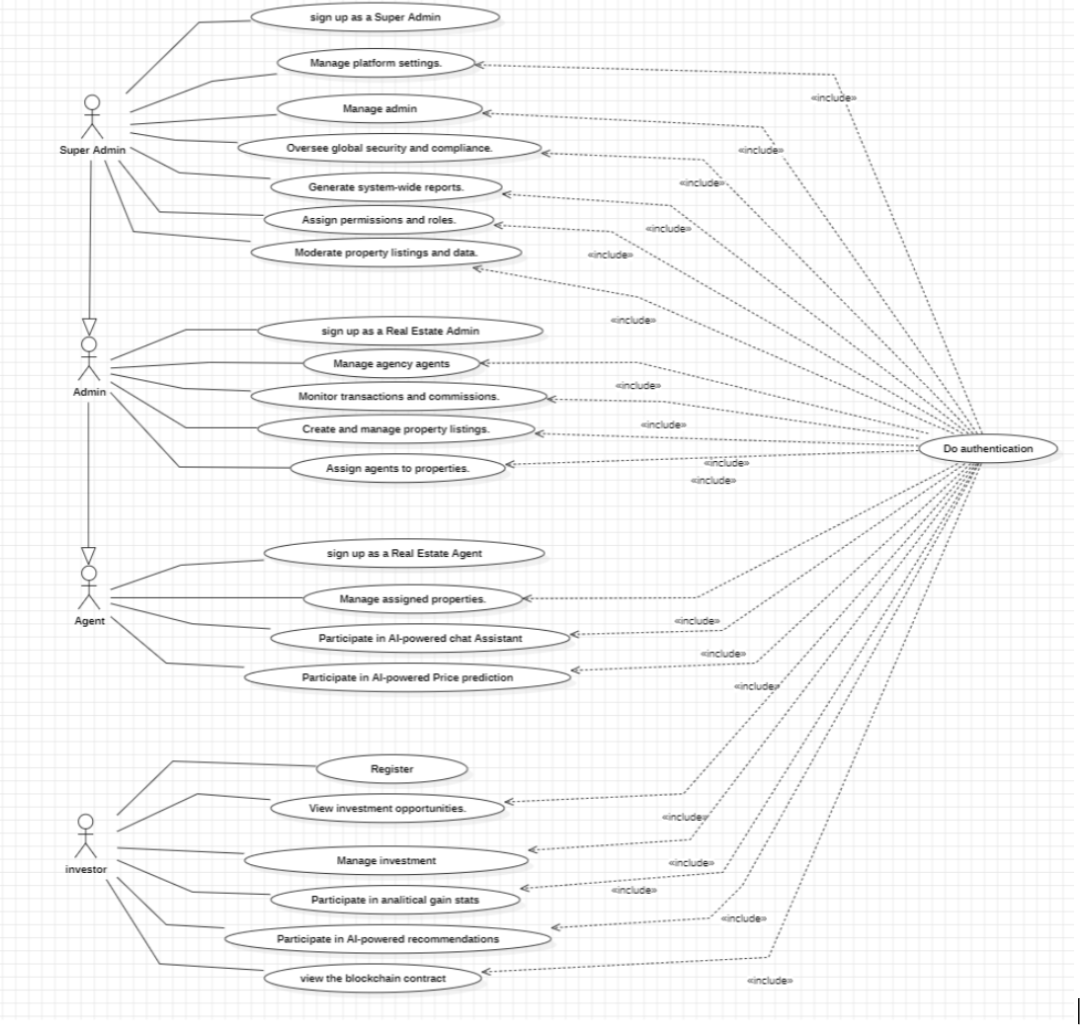
\includegraphics[width=0.6\textwidth]{images/diagram de case d utilisation general.png}
    \caption{General use case diagram}
    \label{fig:use-case-diagram}
\end{figure}
\newpage
\section{Software architecture}

Before starting the design and development of any computerized system, it is essential to prepare the architecture.

\subsection{Physical architecture}

 The physical architecture of Korpor leverages modern, scalable technologies to deliver a seamless investment platform. The frontend is built with Expo, React, and TypeScript using Vite \cite{ViteJSWebsite} for rapid development and Tanstack for robust state management and data visualization, while Storybook supports isolated UI component development \cite{StorybookDocs2022}. The backend relies on Express.js \cite{ExpressJSWebsite} with user authentication managed by Clerk \cite{ClerkAuthenticationDocs}, containerization via Docker \cite{DockerArchitecture2023}, and MySQL \cite{MySQLWebsite} for data storage hosted on Microsoft Azure \cite{AzureCloudServices2024}. Integrated AI modules provide personalized insights \cite{JohnsonAIPropertyValuation2024}, and blockchain technology ensures transactional security and data immutability \cite{WangBlockchainRealEstate2023, McKinseyBlockchainRE2023}. This setup is further supported by GitHub \cite{GithubWebsite} for version control, Postman \cite{PostmanWebsite} for API testing, and end-to-end testing tools like Maestro and Playwright \cite{PlaywrightDocs2023}, with architectural designs and documentation maintained using StarUML \cite{StarUMLWebsite} and Overleaf.

\begin{figure}[htbp]
    \centering
    % Replace with actual image file once available
    % \includegraphics[width=0.85\textwidth]{images/physical_architecture.png}
    \caption{Deployment diagram}
    \label{fig:physical-architecture}
\end{figure}

\subsection{Logical architecture}

To better manage code organization and ensure maintainability, we've designed our application based on the MVC (Model-View-Controller) \cite{SunardiMVC2019, GammaPatterns1994} architectural pattern:

\begin{itemize}
    \item \textbf{Model}: Represents application data and business logic.
    \item \textbf{View}: Presents data to users through interfaces.
    \item \textbf{Controller}: Processes incoming requests, performs operations using Models, and returns appropriate Views.
\end{itemize}

Architecture Components:
\begin{itemize}
    \item \textbf{Model:} The data layer interacts with the backend through ORM or query-based operations, ensuring efficient data retrieval and persistence.
    
    \item \textbf{Controller:} The Express.js backend acts as the intermediary between the database and the frontend, handling user requests, business logic, and data validation. It processes API calls from the frontend and interacts with services such as Clerk for authentication, AI modules for predictive analytics, and blockchain integration for secure transactions.
    
    \item \textbf{View:} The frontend is built with React, TypeScript, and TanStack tools, ensuring a responsive and interactive UI. The frontend communicates with the backend via API requests, displaying dynamic content and allowing seamless user interaction.
\end{itemize}

The logical architecture is illustrated in Figure \ref{fig:logical-architecture}.

\begin{figure}[htbp]
    \centering
    % Replace with actual image file once available
    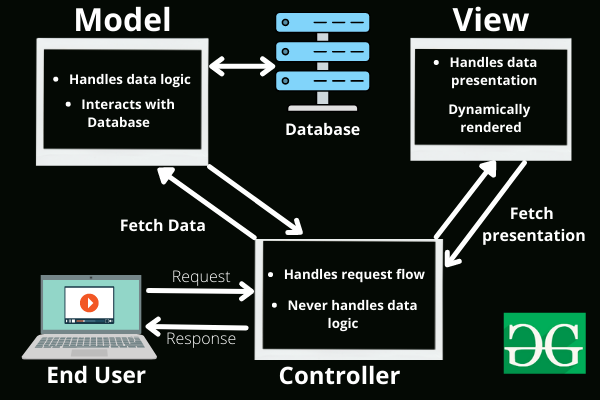
\includegraphics[width=0.9\textwidth]{images/logique.png}
    \caption{Logical architecture}
    \label{fig:logical-architecture}
\end{figure}

Request Flow:
\begin{enumerate}
    \item A user action (e.g., viewing property listings) triggers a request in the frontend.
    \item The request is sent to the backend via an API call.
    \item The Express.js controller processes the request, interacting with the database and other services.
    \item Data is retrieved, processed, and returned as a response.
    \item The frontend updates the UI dynamically based on the received data.
\end{enumerate}

This structured approach ensures a scalable, secure, and high-performance system, optimizing Korpor's real estate investment and management operations \cite{KimDevOpsMethods2018}.

\section{Work Environment}

In this part, we will talk about our work environment, focusing on different aspects:
our material environment, the techniques we used in the realization of our project as well as the tools we used in our report, the product backlog and sprint planning, and finally, we will conclude this section \cite{BeckXP2004, MartinCleanArchitecture2017}.

\subsection{Physical environment}

The work was carried out by a laptop computer that is equipped with these detailed features presented in Table \ref{tab:physical-env} below:

\begin{table}[htbp]
    \centering
    \begin{tabular}{|l|l|}
        \hline
        \textbf{Computer Name} & MSI \\
        \hline
        \textbf{Processor} & i5 10th gen \\
        \hline
        \textbf{Hard disk} & 512 Go SSD \\
        \hline
        \textbf{RAM} & 24.0 Go \\
        \hline
        \textbf{Operating system} & Windows 11 Pro \\
        \hline
    \end{tabular}
    \caption{Physical environment}
    \label{tab:physical-env}
\end{table}

\subsection{Used technologies}

% Define a command for technology icons to make it easier to adjust if needed
\newcommand{\techicon}[1]{%
  \includegraphics[height=1em]{images/icons/#1.png}%
}

\subsubsection*{\protect\techicon{expo} Expo}

Expo is an open-source platform for making universal native apps for Android, iOS, and the web with JavaScript and React.

\subsubsection*{\protect\techicon{typescript} TypeScript}
                                                                
TypeScript (abbreviated as TS) is a free and open-source high-level programming language developed by Microsoft that adds static typing with optional type annotations to JavaScript \cite{TypeScriptDocs2023}. It is designed for the development of large applications and transpiles to JavaScript.

\subsubsection*{\protect\techicon{tanstack} Tanstack}
                                                                      
High-quality open-source software for web developers \cite{TanstackWebsite}. Headless, type-safe, \& powerful utilities for Web Applications, Routing, State Management, Data Visualization, Datagrids/Tables, and more.

\subsubsection*{\protect\techicon{clerk} Clerk}
                                                                        
Clerk \cite{ClerkAuthenticationDocs} is a complete suite of embeddable UIs, flexible APIs, and admin dashboards to authenticate and manage your users.

\subsubsection*{\protect\techicon{maestro} Maestro}
                                                                        
Maestro \cite{MaestroDocs2022} is the simplest, most powerful, and most trusted end-to-end testing platform for mobile and web apps.

\subsubsection*{\protect\techicon{azure} Google cloud platform}

Google cloud platform, or just GCP, is the cloud computing platform developed by Google. It has management, access and development of applications and services to individuals, companies, and governments through its global infrastructure.

\subsubsection*{\protect\techicon{github} GitHub}

GitHub \cite{GithubWebsite} is a cloud-based service that helps developers store and manage their code, as well as track and control changes to their code.

\subsubsection*{\protect\techicon{express} Express.js}

Express.js \cite{ExpressJSWebsite} is a minimal and flexible Node.js \cite{NodeJSWebsite} web application framework that provides a list of features for building web and mobile applications easily.

\subsubsection*{\protect\techicon{postman} Postman}

Postman \cite{PostmanWebsite} is an API platform for building and using APIs. Postman simplifies each step of the API lifecycle and streamlines collaboration so you can create better APIs—faster.

\subsubsection*{\protect\techicon{vite} Vite}

Vite \cite{ViteJSWebsite} is a modern build tool that provides a fast and optimized development experience for React 17 applications. It leverages native ES modules and offers a highly efficient development server with hot module replacement (HMR).

\subsubsection*{\protect\techicon{react} React}

React \cite{ReactWebsite}, sometimes referred to as a frontend JavaScript framework, is a JavaScript library created by Facebook.

\subsubsection*{\protect\techicon{mysql} MySQL}

MySQL \cite{MySQLWebsite} is an open-source relational database management system. It is based on structured query language (SQL), which is used to add, access and manage content in a database.

\subsubsection*{\protect\techicon{docker} Docker}

Docker is an open platform for developing, shipping, and running applications \cite{DockerArchitecture2023}. Docker enables you to separate your applications from your infrastructure so you can deliver software quickly.

\subsubsection*{\protect\techicon{playwright} Playright}

Playwright \cite{PlaywrightDocs2023} is an open-source testing and automation framework that can automate web browser interactions. To put it simply, you can write code that can open a browser \cite{DevOpsFoundation2023}.

\subsubsection*{\protect\techicon{storybook} Storybook}

Storybook is a frontend workshop for building UI components and pages in isolation. It helps you develop and share hard-to-reach states and edge cases without needing to run your whole app \cite{MarcotteResponsiveWebDesign2023}.

\subsubsection*{\protect\techicon{staruml} StarUML}

StarUML \cite{StarUMLWebsite} is a sophisticated software modeler aimed to support agile and concise modeling. It provides eleven different types of diagrams and it accepts UML 2.x standards.

\subsubsection*{\protect\techicon{node} Node.js}

Node.js \cite{NodeJSWebsite} is an open-source, cross-platform JavaScript runtime environment that executes JavaScript code outside a web browser, allowing developers to use JavaScript for server-side scripting.

\subsection{Tools used for the report}

% Comment out problematic icon
\subsubsection*{\protect\techicon{overleaf} Overleaf}

Overleaf is a collaborative cloud-based LaTeX editor used to write, edit, and publish scientific papers.

% Comment out problematic icon
\subsubsection*{\protect\techicon{canva} Canva}

Canva is a global company that empowers people to design anything and publish anywhere. Learn about its mission, values, commitments, awards, product, and careers.

\subsection{Source code management with Git and GitHub}

We used GitHub \cite{GithubWebsite} for storing our application code. We set up a repository with a structured branching strategy to ensure organized development.
\newpage

The main branch maintains the history of official releases, while the develop branch is used for integrating new features. This approach allows us to maintain a stable production version while simultaneously developing new functionality.

\begin{figure}[ht!]
    \centering
    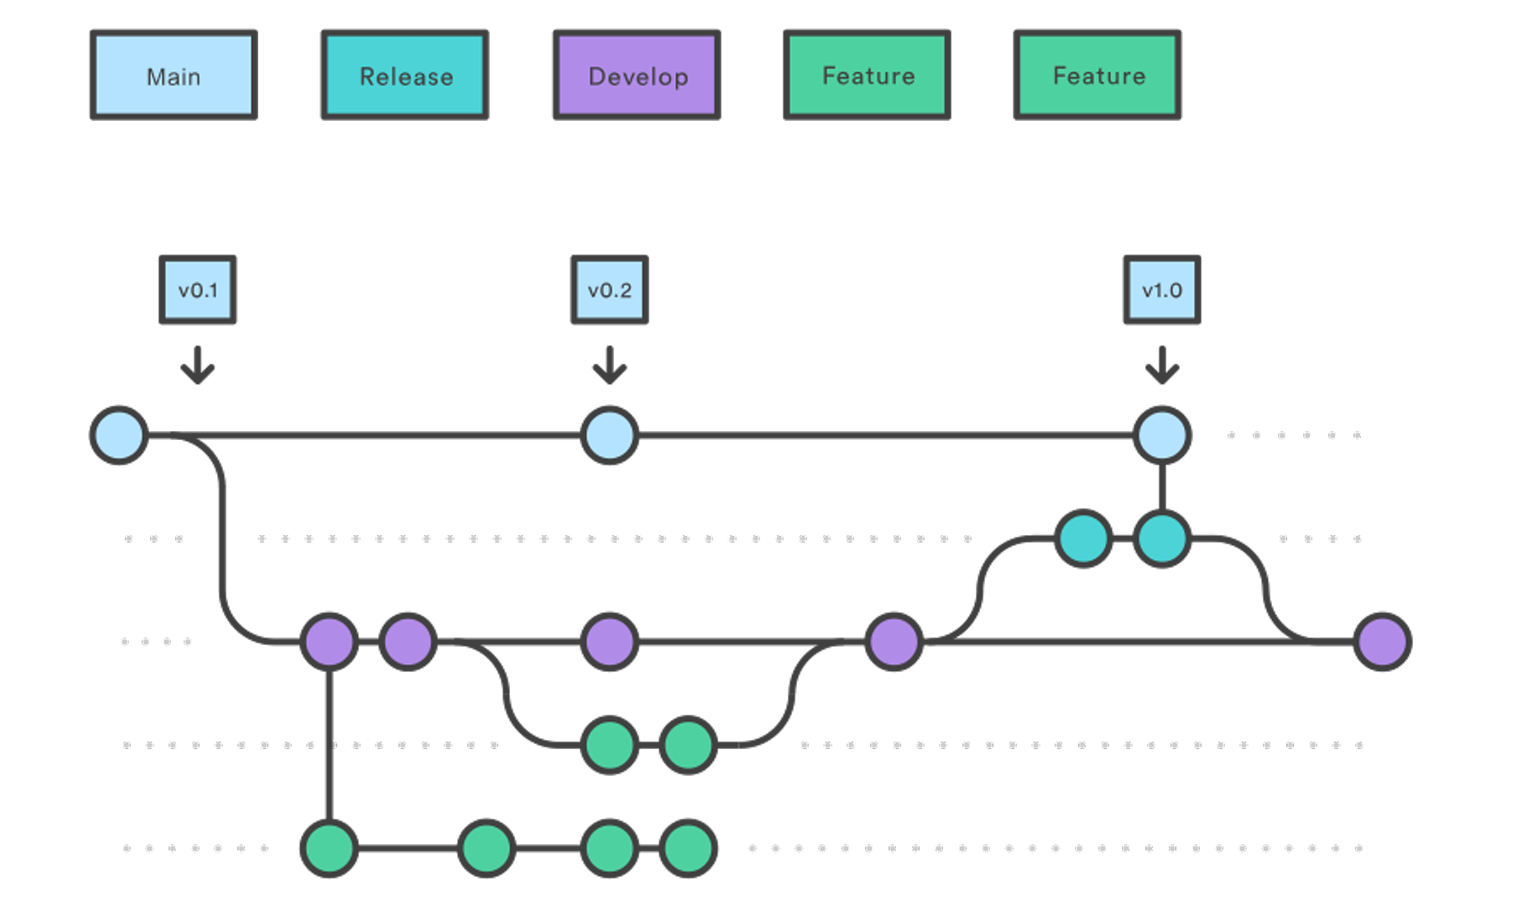
\includegraphics[width=0.9\textwidth]{images/gitWorkflow.png}
    \caption{Git Workflow}
    \label{fig:git-workflow}
\end{figure}

For each new feature or bug fix, we create a feature branch from develop. Once the work is completed and tested, it is merged back into develop through a pull request process. This ensures code review and quality control before any changes are integrated. When a release is ready, develop is merged into main, creating a new stable version of the application.

\section{Product backlog}

The backlog was created before the sprints to plan the milestones and determine the content of each sprint based on project needs \cite{ProductBacklogGuide2024, SchwarzScrum2019}. It includes the following fields:
\begin{itemize}
    \item \textbf{Code:} The unique identifier of the task.
    \item \textbf{Theme:} The subject of a user story.
    \item \textbf{User Story:} A short description of the functionality requested by the client.
    \item \textbf{Priority:} A value indicating the importance of the functionality \cite{MoscowMethodology2021, CleggCaseMethod2004}.
    \begin{itemize}
        \item \textbf{Must:} The feature is essential and must be implemented.
        \item \textbf{Should:} The feature should be implemented if possible.
        \item \textbf{Could:} The feature is optional and may be deprioritized.
        \item \textbf{Won't:} The feature is not a priority at this time.
    \end{itemize}
\end{itemize}

Table \ref{tab:product-backlog} shows the product backlog for our Korpor project:

\begin{longtable}{|c|l|p{8cm}|c|}
    \caption{Korpor Product Backlog\label{tab:product-backlog}} \\
        \hline
        \textbf{Code} & \textbf{Theme} & \textbf{User story} & \textbf{Priority} \\
        \hline
    \endfirsthead
    
    \hline
    \endhead
    
    \hline \multicolumn{4}{|r|}{{Continued on next page}} \\ \hline
    \endfoot
    
    \hline
    \endlastfoot
    
    % Authentication & User Management section
    \multicolumn{4}{|c|}{\cellcolor{primary!15}\textbf{\textcolor{primary}{Authentication \& User Management}}} \\
    \hline
    PB001 & Authentication & As a user, I want to create an account and authenticate securely & Must \\
    \hline
    PB002 & User Management & As a user, I want to manage my profile information & Must \\
    \hline
    PB003 & Authentication & As a user, I want to securely reset my password & Must \\
    \hline
    PB004 & Admin Management & As a Super Admin, I want to manage admin accounts for different real estate companies & Should \\
    
    
    % Super Admin Features section
    \multicolumn{4}{|c|}{\cellcolor{primary!15}\textbf{\textcolor{primary}{Super Admin Features}}} \\
    \hline
    PB005 & Security & As a Super Admin, I want to monitor security and compliance across the platform & Could \\
    \hline
    PB006 & Configuration & As a Super Admin, I want to configure platform-wide features and settings & Could \\
    \hline
    PB007 & Analytics & As a Super Admin, I want to generate and analyze global performance reports & Could \\
    \hline
    PB008 & Moderation & As a Super Admin, I want to moderate content across the platform & Won't \\
    \hline
    PB009 & AI Integration & As a Super Admin, I want to chat with an AI assistant that can securely access database information & Could \\
    \hline
    


    % Admin Features section
    \multicolumn{4}{|c|}{\cellcolor{primary!15}\textbf{\textcolor{primary}{Admin Features}}} \\
    \hline
    PB010 & Listing Management & As an Admin, I want to manage real estate listings in my company & Must \\
    \hline
    PB011 & Agent Management & As an Admin, I want to oversee real estate agents and their permissions & Should \\
    \hline
    PB012 & Transaction Management & As an Admin, I want to track transactions and calculate agent commissions & Should \\
    \hline
    PB013 & Customer Service & As an Admin, I want to address investor inquiries and issues & Could \\
    \hline
    PB014 & Analytics & As an Admin, I want to access a comprehensive agency dashboard & Could \\
    \hline
    PB015 & AI Integration & As an Admin, I want to input property details and receive AI-powered valuation & Should \\
    \hline
    
    % Real Estate Agent Features section
    \multicolumn{4}{|c|}{\cellcolor{primary!15}\textbf{\textcolor{primary}{Real Estate Agent Features}}} \\
    \hline
    PB016 & Listing Management & As an Agent, I want to create and manage property listings & Must \\
    \hline
    PB017 & Investment Management & As an Agent, I want to handle investment and purchase requests & Could \\
    \hline
    PB018 & Data Management & As an Agent, I want to contribute data for AI-driven estimates & Could \\
    \hline
    PB019 & Customer Relations & As an Agent, I want to maintain client relationships and communications & Could \\
    \hline
    PB020 & Finance & As an Agent, I want to view my commissions on sales and rentals & Should \\
    \hline
    
    % Investor Features section
    \multicolumn{4}{|c|}{\cellcolor{primary!15}\textbf{\textcolor{primary}{Investor Features}}} \\
    \hline
    PB021 & Property Discovery & As an Investor, I want to browse available property listings & Must \\
    \hline
    PB022 & Search Functionality & As an Investor, I want to filter properties based on my preferences & Could \\
    \hline
    PB023 & Investment Process & As an Investor, I want to invest in properties through a simple process & Could \\
    \hline
    PB024 & Portfolio Management & As an Investor, I want to track my investment portfolio in real-time & Must \\
    \hline
    PB025 & Payment Processing & As an Investor, I want to make secure payments through various methods & Should \\
    \hline
    PB026 & AI Recommendations & As an Investor, I want to receive personalized property recommendations & Must \\
    \hline
    PB027 & AI Assistance & As an Investor, I want to consult an AI assistant for real estate legal questions & Could \\
    \hline
    PB028 & Financial Prediction & As an Investor, I want to see predictions of potential earnings & Could \\
    \hline
    PB029 & Finance Management & As an Investor, I want to manage my earnings and withdrawals & Could \\
    \hline
    
    % AI & Machine Learning Features section
    \multicolumn{4}{|c|}{\cellcolor{primary!15}\textbf{\textcolor{primary}{AI \& Machine Learning Features}}} \\
    \hline
    PB030 & AI System & As the System, I want to analyze user interactions for personalized recommendations & Must \\
    \hline
    PB031 & AI Prediction & As the System, I want to predict property valuations and rental prices & Should \\
    \hline
    PB032 & AI Forecasting & As the System, I want to forecast potential investment returns & Should \\
    \hline
    PB033 & NLP Integration & As the System, I want to provide real estate legal information via NLP & Could \\
    \hline
    PB034 & Security & As the System, I want to secure AI database access for authorized queries & Could \\
    \hline
    
    % Blockchain & Smart Contract Features section
    \multicolumn{4}{|c|}{\cellcolor{primary!15}\textbf{\textcolor{primary}{Blockchain \& Smart Contract Features}}} \\
    \hline
    PB035 & Blockchain & As the System, I want to create and manage virtual contracts for transactions \cite{WangBlockchainRealEstate2023} & Must \\
    \hline
    PB036 & Blockchain & As an Investor, I want my property investments to be secured via blockchain \cite{McKinseyBlockchainRE2023} & Must \\
    \hline
    PB037 & Blockchain Management & As an Admin, I want to verify and validate blockchain transactions & Should \\
    \hline
    PB038 & Data Integrity & As the System, I want to store transaction records immutably on blockchain & Must \\
    \hline
    PB039 & System Monitoring & As a Super Admin, I want to monitor blockchain health and performance & Should \\
    \hline
    
    % System & Security Features section
    \multicolumn{4}{|c|}{\cellcolor{primary!15}\textbf{\textcolor{primary}{System \& Security Features}}} \\
    \hline
    PB040 & Authentication & As the System, I want to automate authentication and session management & Should \\
    \hline
    PB041 & Notifications & As the System, I want to generate real-time notifications for relevant users & Could \\
    \hline
    PB042 & Data Consistency & As the System, I want to maintain transaction consistency across the platform & Should \\
    \hline
    PB043 & Security & As the System, I want to ensure secure communication between AI and database & Should \\
    \hline
    
    % DevOps & Infrastructure section
    \multicolumn{4}{|c|}{\cellcolor{primary!15}\textbf{\textcolor{primary}{DevOps \& Infrastructure}}} \\
    \hline
    PB044 & CI/CD & As a Developer, I want CI/CD pipelines to build project images on GitHub \cite{ForsgreniDevOpsMetrics2023} & Must \\
    \hline
    PB045 & Deployment & As a Developer, I want to automate image deployment to GCP registry & Must \\
    \hline
    PB046 & Deployment & As a Developer, I want to auto-deploy backend services and database & Must \\
    \hline
    PB047 & Containerization & As a Developer, I want to containerize application components with Docker & Must \\
    \hline
    PB048 & Web Deployment & As a Developer, I want to automatically deploy the web app frontend & Should \\
    \hline
    PB049 & Mobile Deployment & As a Developer, I want to automate mobile app deployments to Play Store & Should \\
    \hline
    PB050 & Versioning & As a Developer, I want to implement versioning for mobile app releases & Should \\
    \hline
    PB051 & Monitoring & As an Admin, I want to monitor system health and performance & Could \\
    \hline
    PB052 & Configuration & As a Super Admin, I want to manage environment configurations & Could \\
        \hline
    
    % Mobile App Specific Features section
    \multicolumn{4}{|c|}{\cellcolor{primary!15}\textbf{\textcolor{primary}{Mobile App Specific Features}}} \\
    \hline
    PB053 & Mobile UI/UX & As an Investor, I want a responsive, intuitive mobile interface \cite{NielsenResponsiveDesign2019} & Should \\
    \hline
    PB054 & Notifications & As an Investor, I want to receive push notifications about my investments & Should \\
    \hline
    PB055 & Offline Access & As an Investor, I want offline access to my basic portfolio information & Should \\
\end{longtable}

\section{Sprint planning}

In order to complete the project within the deadlines set by the internship agreement, planning is an important step in the process \cite{SutherlandScrum2020, RubinEssentialScrum2012}. It was therefore necessary to define the essential steps and estimate the time to be devoted to the completion of the various tasks. To do this, we made a GANTT chart.

In our project management, we opted for the proportional distribution method in order to estimate the costs \cite{CohnAgileEstimating2005, GreningPlanningPoker2002}.
Figure \ref{fig:gantt-chart} shows the Gantt chart that describes the progress of our project:

\vspace{1cm}
\newpage

\begin{figure}[htbp]
    \centering
    % Replace with actual image file once available
    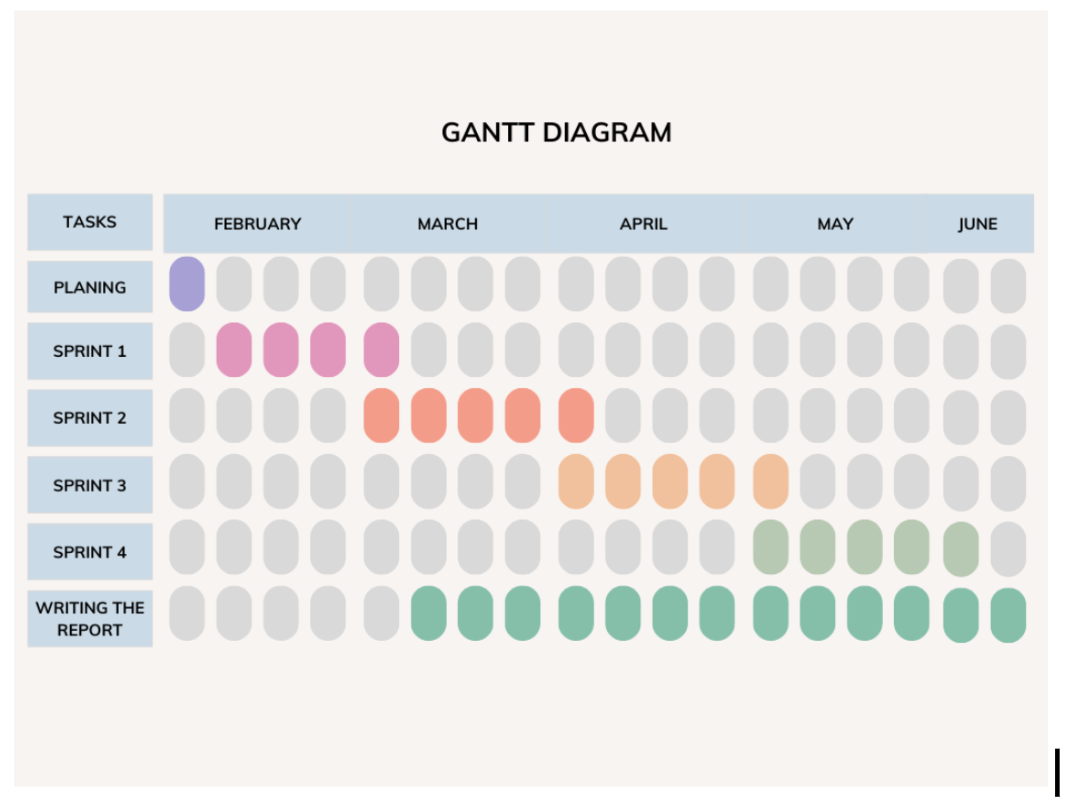
\includegraphics[width=0.7\textwidth]{images/gantt-chart.png}
    \caption{GANTT chart with sprint planning}
    \label{fig:gantt-chart}
\end{figure}

% \vspace{2cm}

\section*{Conclusion}

Our Sprint 0 marked the exciting start of our KORPOR project \cite{ScaledAgileFramework2024, SutherlandScrum2020}. We defined global and specific objectives, developed a solid architecture, and configured an optimal working environment. With a clear vision of the initial product backlog and preliminary planning for upcoming sprints, we are ready to achieve our vision and achieve our goals successfully \cite{SchwarzScrum2019, RubinEssentialScrum2012}.


\cleardoublepage

% Main Matter (Page numbering already set to arabic)
% \chapter{Project Context}
% \input{chapters/project_context.tex}

% \chapter{Introduction} % Example for later
% \input{chapters/introduction.tex}

\end{document} 